\documentclass[conference]{IEEEtran}
\IEEEoverridecommandlockouts
% The preceding line is only needed to identify funding in the first footnote. If that is unneeded, please comment it out.
\usepackage{cite}
\usepackage{amsmath,amssymb,amsfonts}
\usepackage{algorithmic}
\usepackage{graphicx}
\usepackage{textcomp}
\usepackage{xcolor}
\usepackage{subcaption}
\usepackage{flushend}
\def\BibTeX{{\rm B\kern-.05em{\sc i\kern-.025em b}\kern-.08em
    T\kern-.1667em\lower.7ex\hbox{E}\kern-.125emX}}
\begin{document}

\title{Flight Test of a Collision Avoidance Neural Network with Run-Time Assurance
%{\footnotesize \textsuperscript{*}Note: Sub-titles are not captured in Xplore and
%should not be used}
%\thanks{Identify applicable funding agency here. If none, delete this.}
}

\author{\IEEEauthorblockN{Darren Cofer, Ramachandra Sattigeri, \\
Isaac Amundson, Junaid Babar, \\
Saqib Hasan}
\IEEEauthorblockA{\textit{Collins Aerospace} \\
\{first.last\}s@collins.com}
\and
\IEEEauthorblockN{Eric Smith, \\
Karthik Nukala}
\IEEEauthorblockA{\textit{Kestrel Institute} \\
\{eric.smith, nukala\}@kestrel.edu}
\and
\IEEEauthorblockN{Denis Osipychev, Lucca Timmerman, \\
Dragos D. Margineantu, James L. Paunicka, \\
Matthew A. Moser}
\IEEEauthorblockA{\textit{Boeing} \\
\{first.mi.last\}@boeing.com}
}

\maketitle

\begin{abstract}
%Aircraft systems have requirements for airworthiness certification that present barriers to the use
%of machine learning technologies such as neural networks. Showing that a component or system is
%correct and does no harm through behaviors that were unintended by designers or unexpected by
%operators is a critical aspect of the certification process. 
Our team is developing assurance
technologies that can support the use of machine learning in the design of safety-critical aircraft
systems. These capabilities have been integrated on Boeing’s autonomy demonstrator aircraft to show
that they can provide evidence of correct operation and safety guarantees needed by real aircraft.
We have applied run-time assurance along with formal methods modeling and analysis tools to an
airborne collision avoidance system based on a neural network. This system was demonstrated
in-flight and shown to correctly monitor neural network operation and intervene when needed to
prevent violation of the “remain well clear” safety requirement relative to an intruder aircraft.
\end{abstract}

\begin{IEEEkeywords}
machine learning, run-time assurance
\end{IEEEkeywords}

\section{Introduction}

Aircraft systems have requirements for airworthiness certification that present barriers to the use
of machine learning technologies such as neural networks. Showing that a component or system is
correct and does no harm through behaviors that were unintended by designers or unexpected by
operators is a critical aspect of the certification process. In a typical machine learning
application, much of the complexity and design information resides in its training data rather than
in the actual models or software produced. This means that it is generally not possible to determine
the correctness of a neural network by examining its implementation or tracing specific design
elements back to requirements.

Our team is developing assurance technologies that can support the use of machine learning in the
design of safety-critical aircraft systems. These capabilities have been integrated on Boeing’s
autonomy demonstrator aircraft to show that they can provide evidence of correct operation and
safety guarantees needed by real aircraft. In previous work \cite{dasc2020} we have used a run-time assurance
architecture (RTA) to ensure the safety of an autonomous neural network-based aircraft taxiing
application. In our current work we have applied run-time assurance along with formal methods
modeling and analysis tools to an airborne collision avoidance system based on a neural network.
This system was demonstrated in-flight and shown to correctly monitor neural network operation and
intervene when needed to prevent violation of the “remain well clear” safety requirement relative to
an intruder aircraft. Thirty-six test conditions were flown with various collision course
geometries, with relative heading angles of 45, 90, 135, 180 (head-on), 225, 270, and 315 degrees
leading to a pending collision, to test the robustness of the neural net trajectory generator and
the RTA mitigations.

The RTA architecture includes a run-time monitor that provides an independent assessment of the
avoidance flight plans generated by the neural network and a safe (but less optimal) backup planner.
The results of the assessment are evaluated by a decision logic component which selects (based on a
tabular specification of safety rules) a flight plan that will ensure safe flight. The core decision
logic code is synthesized from a formal specification, with most of the synthesis steps producing
machine-checked proofs of their correctness. The RTA architecture has been modeled in the
Architecture Analysis and Design Language (AADL) and formally analyzed to show that it maintains the
system safety requirements.

Autonomous remain-well-clear and collision avoidance capabilities are critical to safe flight of
military and commercial uncrewed aircraft. These autonomous capabilities can also be valuable for
enhancing the safety of flight for piloted aircraft by providing pilot cueing. Run-time assurance
approaches, with run-time monitoring of machine learning software functions integrated with
contingency management functionality, will enable safe use of neural networks in bringing
breakthrough autonomy capabilities to aircraft.

In this paper we will discuss: 
\begin{itemize} 
\item The assurance challenges for the use of neural networks in safety-critical aircraft applications 
\item The autonomy framework and aircraft used to demonstrate the collision avoidance neural network capability 
\item The run-time assurance architecture developed to guarantee the absence of unintended behavior resulting from the neural network 
\item The formal methods assurance technologies applied within the architecture, including analysis of the architecture design and synthesis of decision logic from a formal specification
\item Flight testing, results obtained for various test scenarios, and lessons learned from the
demonstration
\end{itemize}

% motivation
% aerospace applications
% barriers - requirements, verification, coverage and unintended functionality
% brief description of the demo application and clear statement of our accomplishments

\section{Assurance Challenges}

The assurance challenges for the use of neural networks in safety-critical aircraft applications [DARREN]

Show absence of unintended functionality -- do no harm
% Assurance Challenges
% The assurance challenges for the use of neural networks in safety-critical aircraft applications [DARREN]
% show absence of unintended functionality -- "do no harm"

\section{Autonomy Framework}

Overview

\subsection{Autonomy Testbed Aircraft}

%[MATT/JIM] Overview of the Boeing autonomy framework and aircraft used to demonstrate the collision avoidance neural network capability.

%Collision avoidance problem -- Strategic rather than tactical, avoidance flight plan must avoid intruder but return to original flight plan

%Limitations --  two-dimensional, lateral avoidance maneuvers, focus on single intruder

%Describe the safety requirements for collision avoidance.  Maybe reference DO-365. 

The Boeing Autonomy Testbed Aircraft is a Cessna Caravan 208B, tail number N208BX (Figure~\ref{fig:caravan}).  This platform is currently serving as a test bed for the DARPA Assured Autonomy program air domain experiments.  The Testbed is optionally piloted and serves as a means to demonstrate commercially viable technologies leading to autonomy.  It is a research and development vehicle able to operate in commercial airspace that is built on open-source middleware with in-house developed guidance and control technologies leveraged from across the Boeing enterprise.  The Testbed includes a full ``Iron Bird'' fixture for hardware-in-the-loop evaluation in which new autonomy technology can be fully integrated and tested before flight.  With this Testbed Boeing has demonstrated autonomy firsts including in-air detect and avoid, ADS-B transponder-based route planning for strategic avoidance, and fully autonomous ground taxi.

\begin{figure}
	\centering
	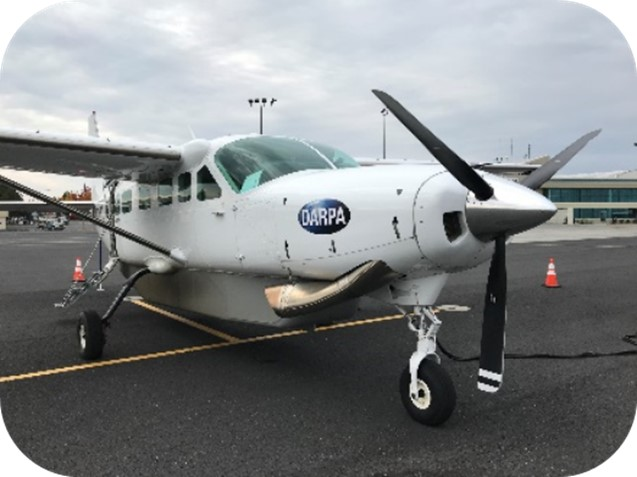
\includegraphics[width=\columnwidth]{figures/caravan.jpg}
	\caption{Boeing Autonomy Testbed Aircraft, Cessna Caravan 208B}
	\label{fig:caravan}
\end{figure}

Detect and avoid (DAA) mission operating and performance standards are defined in RTCA document DO-365 \cite{DO_365}.  The standard provides guidance for interactions of Unmanned Aircraft Systems (UAS) in the National Airspace System, requirements for safe operation of aircraft during encounters including separation distance minimums for remaining well clear of aircraft and avoiding mid-air collisions, and proper aircraft equipage to achieve safe detect and avoid operations.
The assurance challenge posed in our work focuses on the Autonomy Testbed aircraft flying in the vicinity of another ``intruder'' airplane, where the test flight software includes a Boeing-developed LEC to generate an avoidance flight plan for the Testbed to remain well clear of the intruder aircraft as defined in DO-365.  The underlying assurance technology montors the Boeing LEC in order to assess the avoidance trajectory from the LEC and guarantee safety. 

\begin{figure*}
	\centering
	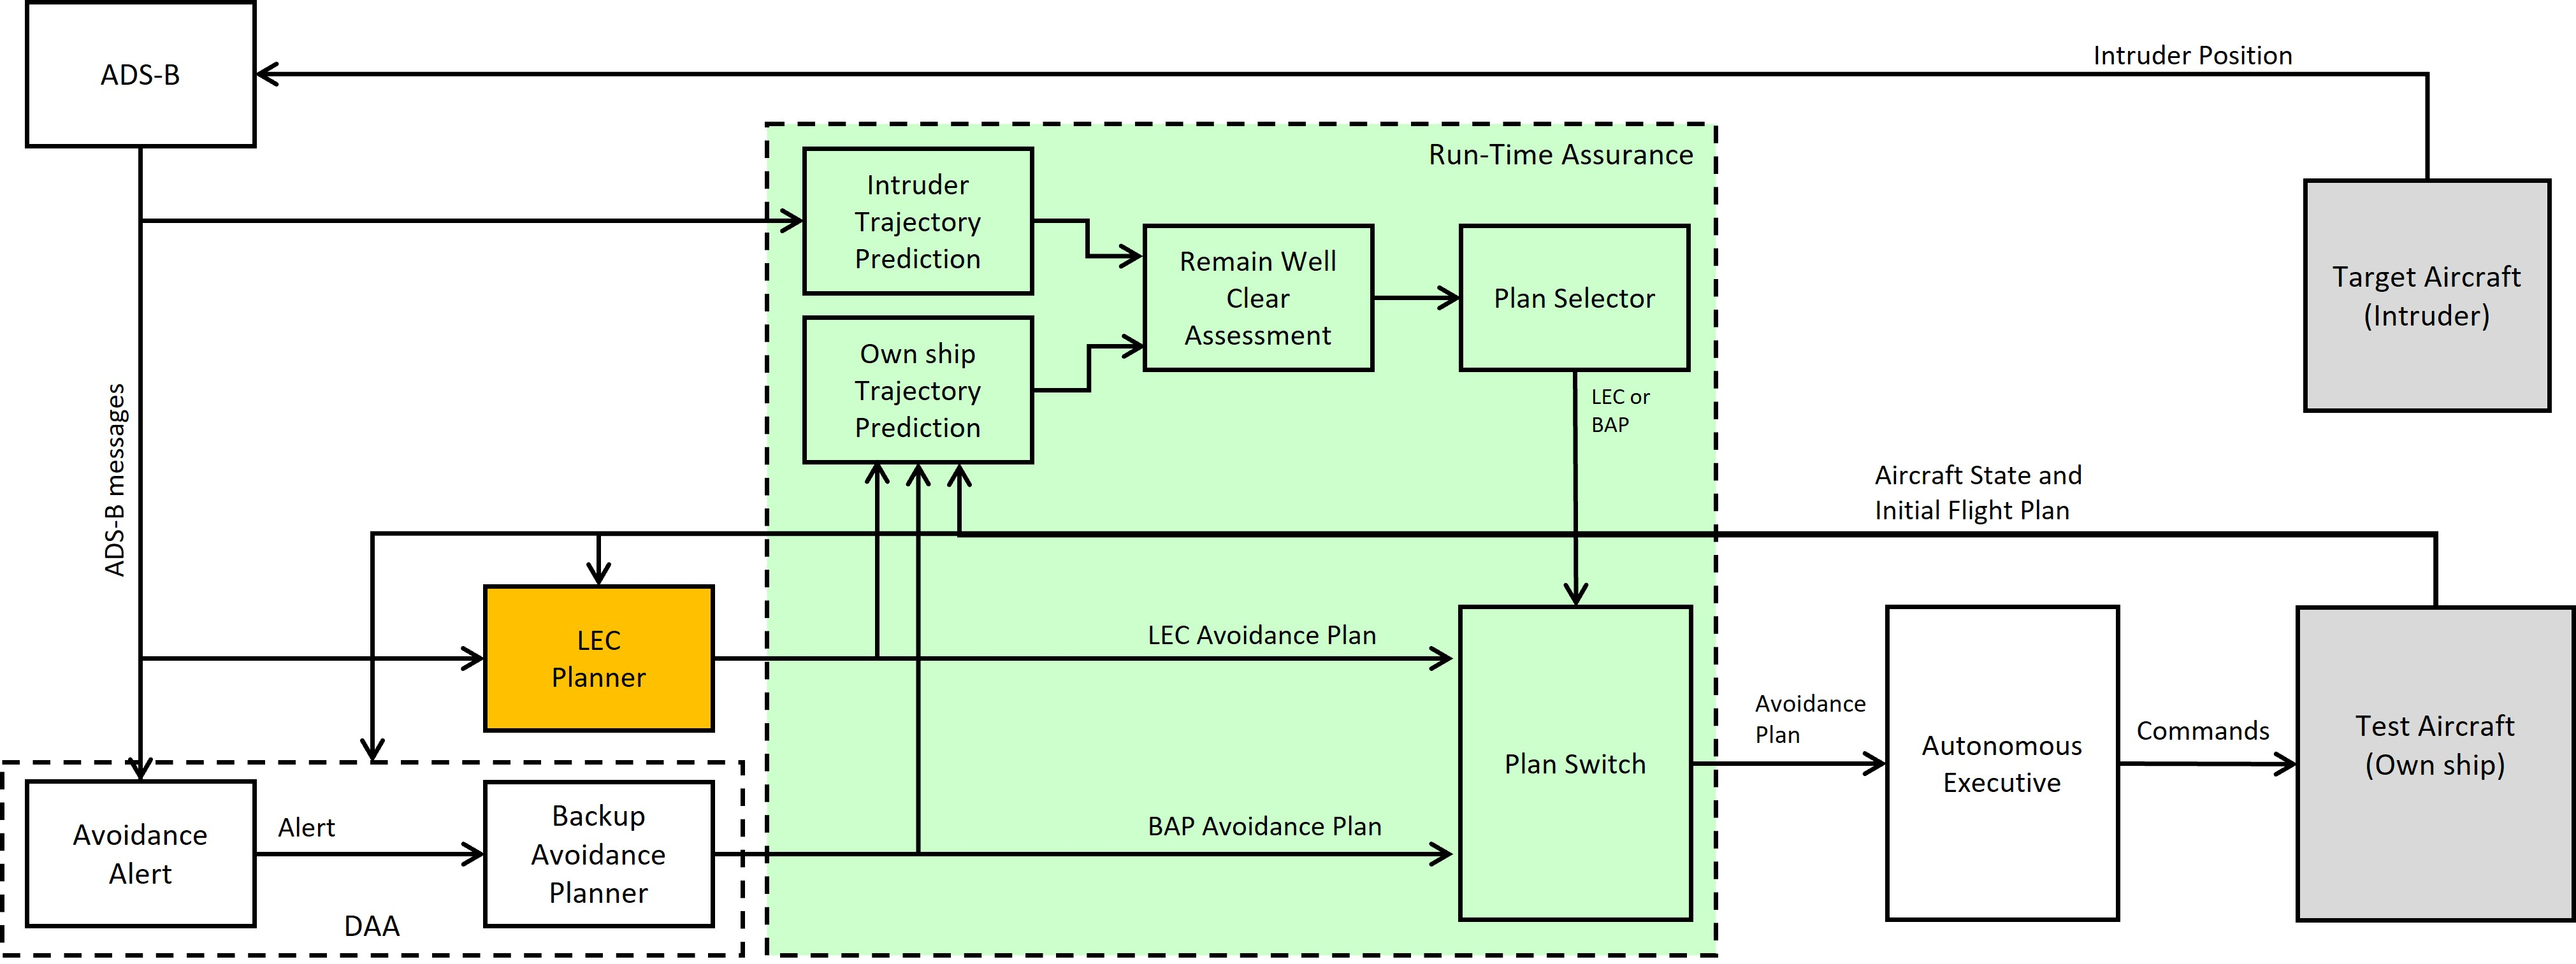
\includegraphics[width=\textwidth]{figures/rta-arch.jpg}
	\caption{Collision avoidance system on the autonomy testbed aircraft with run-time assurance components in green}
	\label{fig:rta-arch}
\end{figure*}

Figure~\ref{fig:rta-arch} shows a block diagram of the autonomy system framework as deployed on the Testbed aircraft.
System elements include: 
\begin{itemize}
\item ADS-B – The primary sensor for perceiving the airspace is the Automated Dependent Surveillance Broadcast (ADS-B) system providing detection information on  nearby aircraft (intruders) to the other system functions.
%\item ADS-B Tracker – Generates intruder track information from received ADS-B messages to the other system functions.
\item Avoidance Alerts – Evaluates potential future traffic conflicts and issues “alerts” to the Avoidance functions.  Assessment definition and requirements are specified in DO-365 MOPS for DAA System.
\item LEC Planner -- Neural network system trained offline through reinforcement learning to generate avoidance flight plans satisfying DAA requirements.  Training and operation is described in the following subsection.  
\item Backup Avoidance Planner – A trusted but less optimal backup planner that provides waypoint navigation paths to avoid airspace incursion.  Avoidance computation method is virtual predictive radar which is designed to provide maximum ``safe passage timed corridors.''  Avoidance path terminates back on the original flight plan.
\item Run-Time Assurance  – Run-time monitoring, predication, and assessment systems that guarantee the selection of a safe flight plan for the aircraft.  Operation and assurance are described in Sections \ref{sec:rta} and \ref{sec:assurance}.
\item Autonomous Executive – Constructs and manages execution of the vehicle flight plan and contains a function to ``splice in'' avoidance guidance waypoint plans into the original flight plan.
%\item Vehicle Manager – Executes flight path provided by AE including guidance and control for the vehicle.  The VM also sends commands and receives feedback from actuation system components.
%\item Actuators / Sensors – Carries out VMS flight control surface commands and provides positional feedback.
%\item Ownship State Estimation – Provides vehicle state information including position, altitude, and speed along with the vehicle inertial reference frame.
%\item Navigation Database – Reference database of aircraft parameters and airspace waypoints, terrain, airports, approaches, etc.  Used for route/avoidance planning purposes.
\end{itemize}



\subsection{LEC Training with Reinforcement Learning}
%Description of LEC and RL, ROS integration

In this work, the corrective maneuver for the avoidance is generated by a pre-computed solution -- Reinforcement Learning (RL) policy model. 
The RL is a sequential policy optimization method that solves the task using the ''learning by doing'' conception and requires continuous data-rich interaction with the environment \cite{sutton2018reinforcement}. 
Our avoidance policy is trained on a surrogate task to provide a required number of interactions. 
This surrogate environment developed by Boeing is a lightweight Python environment integrated with the OpenAI GYM framework \cite{brockman2016openai}.

The learned policy minimizes the risk of collision by providing continuous control commands in the surrogate environment. These commands are converted into a geometric trajectory using the surrogate environment and Boeing-provided ROS interfaces.

\begin{figure}[h]
	\centering
	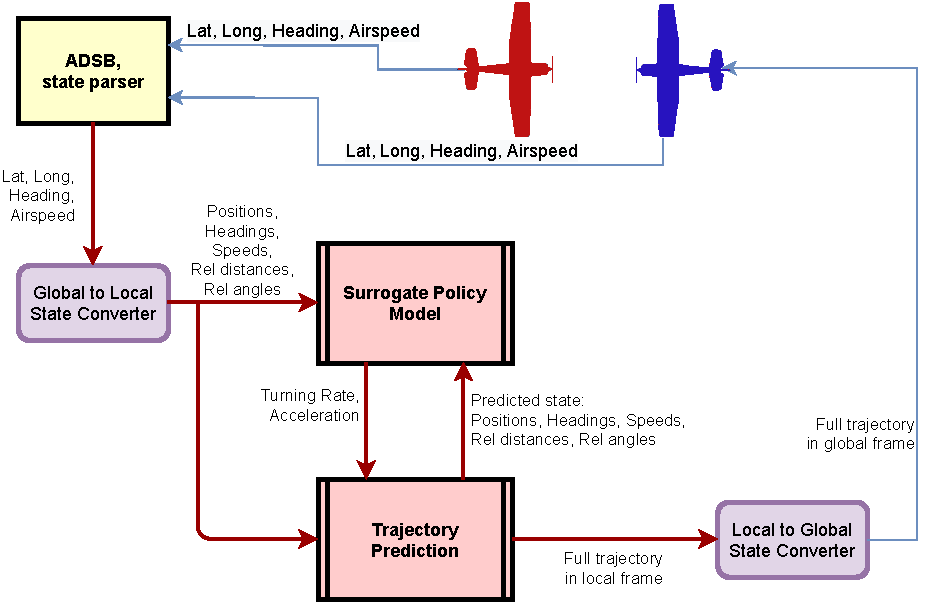
\includegraphics[width=\linewidth]{figures/system_overview.pdf}
	\caption{System diagram of the RL model-based conflict resolver.}
	\label{fig:diagram}
\end{figure}


Our surrogate environment is a simplified 2D obstacle avoidance problem that mimics the real task (air traffic conflict resolution). 
The environment simulates the movements of two aircraft on 20x20 kilometers square. The controlled Agent has to go around the Intruder, provide minimal horizontal separation, and merge back to the next safe waypoint from the original route before the simulation ends.

\begin{table}[h]
	\centering
	\begin{tabular}{||c | c | c||} 
		\hline
		Parameter & Range & Units \\
		\hline
		Time step $dT$ & 1.0  & sec \\
		Max time $t_\text{MAX}$ & 300.0  & sec \\
		Distance range & -10000 .. 10000  & m \\
		Horizontal separation & 1000  & m \\
		\hline
	\end{tabular}
	\caption{Surrogate environment simulation parameters.}
	\label{tbl:sim_param}
\end{table}


The surrogate dynamics imitate the dynamics of the vehicle selected for the experiment -- a single-engine turboprop Cessna 208 Grand Caravan.

All the vehicles are represented by a simplistic dynamic model:
\begin{itemize}
	\item Dubin's vehicle model for turn dynamics
	\item Mass-less kinematics model 
	\end {itemize}
	
	
	All the observation and control values are normalized to [-1..1] for the RL agent.
	
	To make sure the agent generalizes the problem, we rewrap the observations and focus only on relative positions rather than absolute. In addition, we normalize the values to [-1 .. 1].
	Repacked observations consumed by the agent:
	\begin{center}
		\begin{tabular}{|| c | c ||} 
			\hline
			heading & intruder heading\\
			airspeed & intruder airspeed\\
			distance to goal & distance to intruder\\
			tracking angle to goal & tracking angle to intruder\\
			\hline
		\end{tabular}
	\end{center}

\subsection{RL Policy Agent}

The RL policy agent learns the task by interacting with the simulation and iteratively updating the parameters of the policy model using Stochastic Gradient Descent (SGD) optimization. We approximate the policy with a multi-layered perceptron shown in Fig. \ref{fig:policy_model}.

\begin{figure}[h]
	\centering
	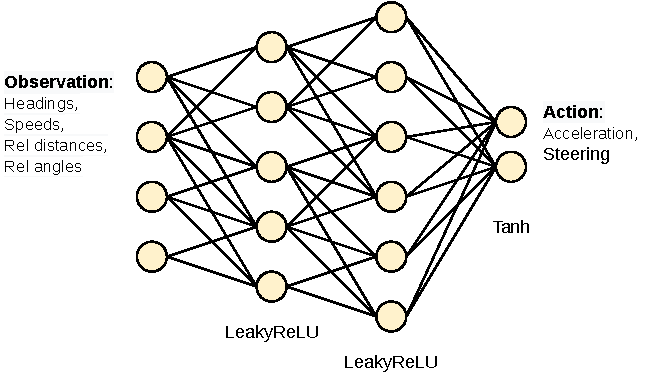
\includegraphics[width=0.7\linewidth]{figures/model.pdf}
	\caption{Neural network function approximation used for the policy model consists of 2 hidden layers, 256 neurons each.}
	\label{fig:policy_model}
\end{figure}

To solve the optimization problem as Markov Decision Problem (MDP) system, we refactor it into Markovian states $s$, transitions  $T(s' | s, a)$, and transition reward $R(s' | s, a)$. 
The state of the system (including both Agent and Intruder) is fully observable, assumes the perfect knowledge, and is enough to describe the Markovian state of the MDP system.
State of the agent described as
$$ s = \{ v_a, \psi_a, v_i, \psi_i, \beta_i, d_i, \beta_g, d_g \}$$

where 
$v_a$ - agent speed,
$\psi_a$ - agent heading,
$v_i$ - intruder speed,
$\psi_i$ - intruder heading,
$\beta_i$ - angle to intruder,
$d_i$ - distance to intruder,
$\beta_g$ - angle to goal,
$d_g$ - distance to goal. 

The optimization is set to find the optimal policy $\pi^*(s)$ as a set of state-action mappings that maximizes the expected reward $V(s)$ \cite{sutton2018reinforcement}.
\begin{align} 
	\pi(s) &= P(a | s) \\
	\pi^*(s) &= \arg\max_{\pi} V^\pi (s) \\
	&= \arg\max_a \left( R(s,a) + \gamma T(s'|s,a) V(s') \right)
\end{align} 

Value of the state is expected future reward accumulated over the trajectory and defined by Bellman function as:
\begin{align}
	V(s) &=  \mathbb{E} [R | s, \pi] \\
	&= \sum_{s'} T(s'|s,a) \left( R(s'|s,a) + \gamma ( V(s')) \right) \\
	&=  R(s'|s,a) + \gamma \sum_{s'} T(s'|s,a) V^{\pi}(s') \\
	V^{*}(s) &= \max_{a} \left( R(s,a) + \gamma \sum_{s'} T(s'|s,a) V^{*}(s') \right)
\end{align}

The RL policy model is based on the Actor-Critic architecture that helps to improve the stability of the training \cite{sutton2018reinforcement}. The SGD-based update for Actor $\theta$ and Critic $w$ networks:
\begin{align}
	\delta &=  R_{t+1} +\gamma \hat V(s_{t+1},w) - \hat V(s_t,w) \\
	w &\leftarrow w + \alpha \delta \nabla \hat V (s, w) \\
	\theta &\leftarrow \theta + \alpha \delta \nabla \ln \pi (a|s, \theta)
\end{align} 

The core functionality of the RL agent incorporates the Stable Baselines library, a very reputable fork of OpenAI Baselines \cite{hill2018stable}. For the exploration policy and update steps, this work used the Proximal Policy Optimization (PPO) algorithm that becomes the state of the art in continuous-action agents \cite{schulman2017proximal}.



[DENIS/DRAGOS]

\subsection{ROS Integration}

\begin{figure}[h]
	\centering
	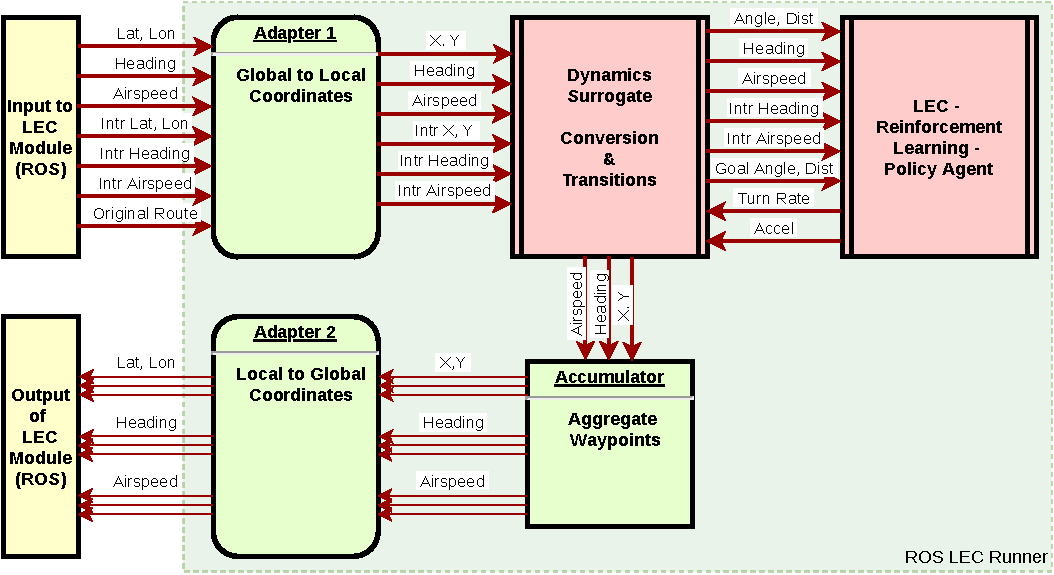
\includegraphics[width=\linewidth]{figures/cp25_ros.pdf}
	\caption{System diagram of the ROS-LEC (ROS-Agent) runner -- the integration of the learning-enables component (LEC) to the physical demonstrator using ROS interface.}
	\label{fig:integration}
\end{figure}

CAS system integration is done using Robot Operating System (ROS) interface \cite{quigley2009ros}. This allows unifying the interfaces to the high-fidelity simulation and to the physical demonstrator.
ROS-Agent (ROS-LEC) runner, demonstrated in Fig. \ref{fig:integration}, aggregates data from different domains and provides important utilities to the system. Its job is designed as follows: 
\begin{itemize}
	\item receive and accumulate ROS messages regarding the own-ship state,
	Intruder's state, traffic alerts, GPS-SRS transformation data,
	\item translate ADSB and GPS-Novatel positioning data to local coordinate frame,
	\item extract the goal location from the original route,
	\item re-wrap the observations into the Agent-specific input format,
	\item iteratively run the Agent to get the corrective actions,
	\item iteratively run the surrogate environment to receive the transitions,
	\item form a corrective trajectory and check if the trajectory is good,
	\item translate the trajectory from local coordinate frame to global lat-long waypoints,
	\item publish the trajectory as ROS message.
\end{itemize}

On an external request, the runner generates a single avoidance trajectory and publishes it as ROS message. The trajectory consists of 20 waypoints in total. The last waypoint is taken from the original route, and 19 waypoints are generated by the policy. This allows linking the waypoints by a unique index and preserving the indices of the original route.

These waypoints are spaced 20 seconds apart which provides a 400-second planning horizon. 
Because of the large time step between the waypoints, the policy and the surrogate have to be evaluated 20 times to make a single waypoint. The total response time of the system is below 60 msec for the complete trajectory.

When needed to re-plan, the runner can be requested again. This architecture allows closed-loop corrections with an external run-time assurance monitor. The monitor keeps track of the accumulated transition error and either requests an updated avoidance plan or denies the operation switching to a back-up mode.

% Autonomy Framework [MATT/DENIS]
% The autonomy framework and aircraft used to demonstrate the collision avoidance neural network capability.
% Safety requirements
% Reinforcement learning and the LEC produced for collision avoidance.
% Execute LEC repetitively to generate avoidance trajectory.

\section{Run-Time Assurance}

[DARREN - 1.5 pg]

Run-Time Assurance Architecture, monitors, high-assurance components, ASTM F3269-17 standard [DARREN]

The run-time assurance architecture developed to guarantee the absence of unintended behavior resulting from the neural network

- RTA, AADL model [DARREN/ISAAC]

- Trajectory prediction, SWC assessment [RAM/DARREN]

% Run-Time Assurance Architecture, monitors, high-assurance components, ASTM F3269-17 standard
% The run-time assurance architecture developed to guarantee the absence of unintended behavior resulting from the neural network
% - RTA, AADL model [DARREN/ISAAC]
% - Trajectory prediction, SWC assessment [RAM/DARREN]

\section{Assurance Technologies}
\label{sec:assurance}

[DARREN - 3 pg total for section]

The formal methods assurance technologies applied within the architecture, 
including analysis of the architecture design and synthesis of decision logic from a formal specification

% Subsections
% - AGREE
% - Resolute
% - Logic

% Assurance Technologies
% The formal methods assurance technologies applied within the architecture,
% including analysis of the architecture design and synthesis of decision logic from a formal specification

\subsection{Architecture Verification}

%AGREE analysis of RTA arch in AADL

One of the steps for design-time assurance of the RTA architecture is verifying the architecture satisfies its high-level requirements.  Traditionally, requirements verification has been achieved using a combination of directed testing methods and manual review. However, model-based specification enables a more rigorous approach to verification via formal methods analysis. With both the requirements and architecture represented in formal (well-defined, unambiguous) notations, SMT solvers can be employed to determine whether there is any possible sequence of inputs that will violate a requirement.  Furthermore, failure by the solver to find a counterexample is essentially equivalent to a mathematical proof that the requirement can never be violated.  

In architecture models, we can represent high-level requirements as assume-guarantee contracts on components.  \textit{Guarantees} are statements about a component's outputs which will always hold as long as stated \textit{assumptions} are valid.  When designing an architecture comprised of multiple components, it is imperative to verify that a system's subcomponent contracts satisfy the overall system contract, as well as whether a component's assumptions are valid with respect to the specified upstream guarantees and environment.
%
We use the AGREE tool~\cite{agree2012} to specify and analyze component contracts in our run-time assurance architecture.  AGREE is a plugin for the Open Source AADL Tool Environment (OSATE), enabling contracts to be specified directly on AADL model components and analyzed within the modeling environment.

%The RTA architecture was modeled in AADL (Figure~\ref{fig:rta-agree}) using the Open Source AADL Tool Environment (OSATE), and the high-level requirements were added to this AADL model as AGREE specifications \cite{agree2012}.  AGREE specifications are used to describe component behavior through assume-guaranteee contracts, and these contracts are analyzed using AGREE's compositional reasoning framework available through the AGREE plugin for OSATE.

The main objective of our AGREE analysis of the collision avoidance model was to verify that the RTA architecture is guaranteed to publish only safe flight plans.
%
%In Figure~\ref{fig:rta-agree}, when an avoidance alert is generated, the Safe Backup Planner generates a BAF plan; this triggers the generation of an LEC plan. The Plan Selector chooses one of the two plans based on the SWC Assessment output, and informs the Plan Switch of its decision. The Plan Switch publishes a flight plan based on the Plan Selector output.
As illustrated in Figure~\ref{fig:rta-agree}, we annotated the AADL model with assume-guarantee contracts for each component in the architecture, and AGREE was able to verify the high-level property under the assumption that BAF flight plan is always safe.

\begin{figure*}
	\centering
	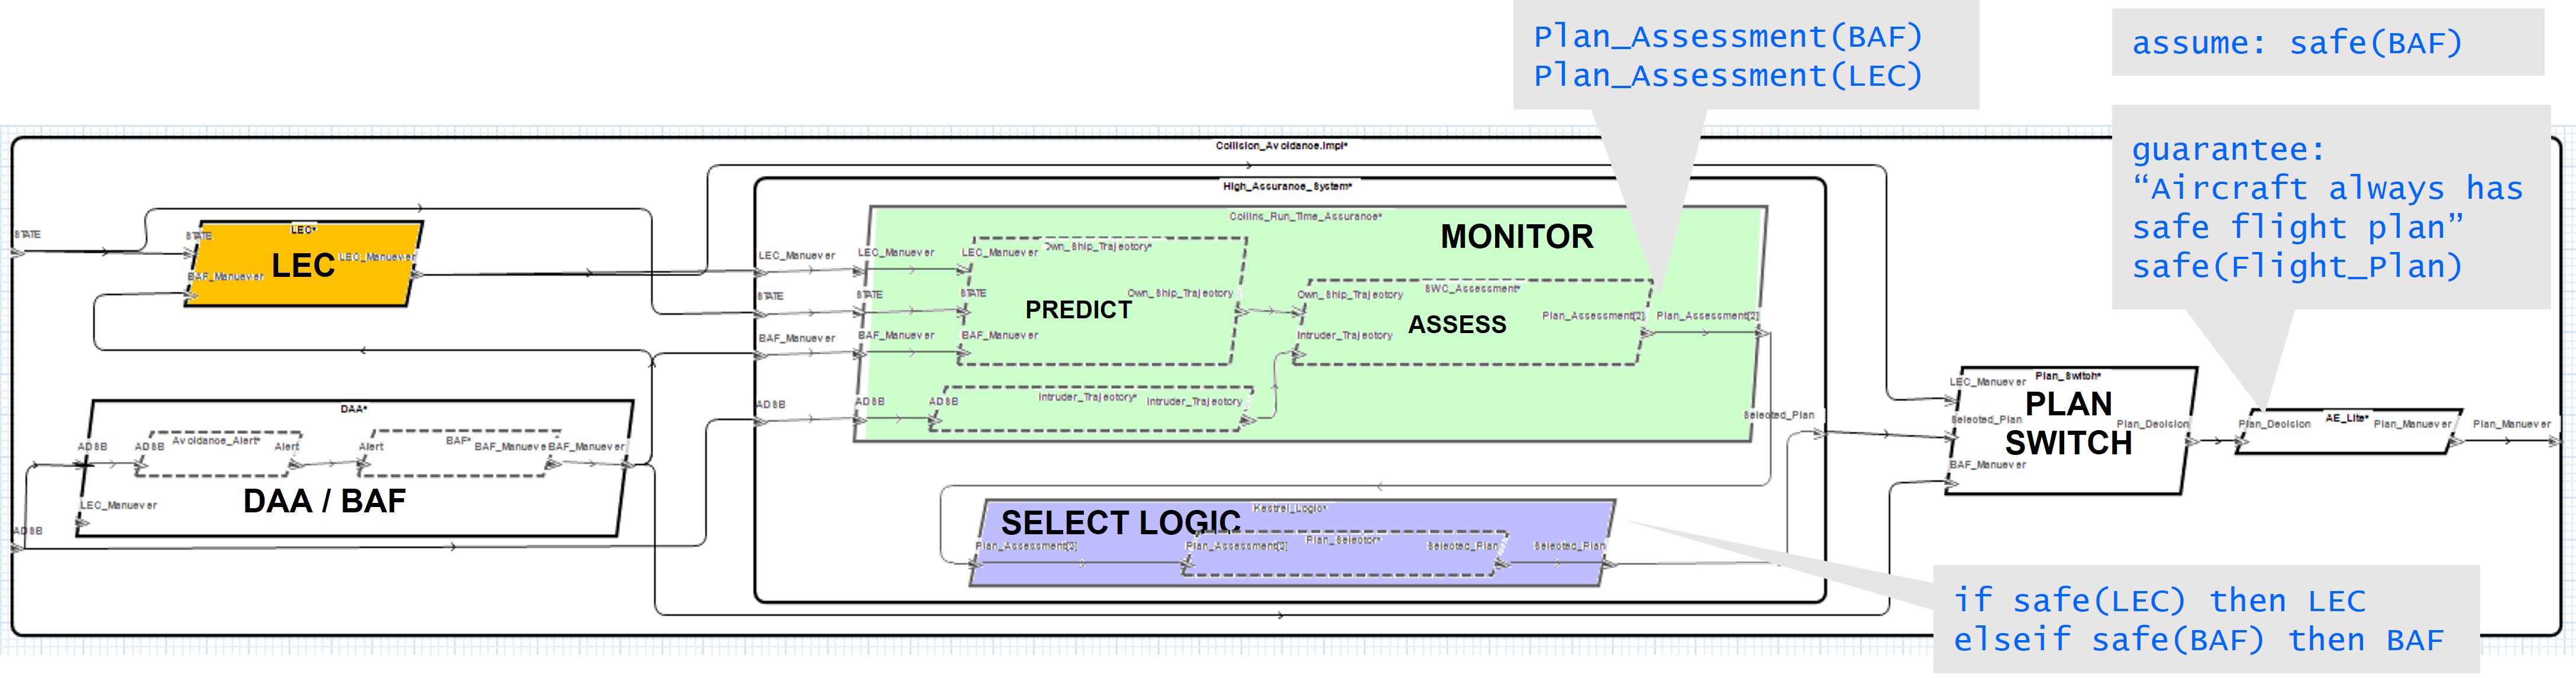
\includegraphics[width=\textwidth]{figures/rta-agree.jpg}
	\caption{AADL Model of Run-Time Assurance Architecture and AGREE properties}
	\label{fig:rta-agree}
\end{figure*}
% - AGREE analysis of RTA arch in AADL [JUNAID/ISAAC]

\subsection{Decision Logic}

[ERIC/KARTHIK - 1 pg]
 
Decision logic, tabular spec and evolution, APT synth and proof

% - Decision logic, tabular spec and evolution, APT synth and proof [ERIC/KARTHIK]

\subsection{Assurance Argument}

[SAQIB/ISAAC - 1 pg]

Resolute Assurance argument for RTA arch

% - Resolute Assurance argument for RTA arch [SAQIB/ISAAC]

\section{Flight Test Results}

%[DARREN/JIM - 1.5 pg]
Our flight testing plan evaluated the performance of the LEC collision avoidance planner and the RTA architecture using the Boeing Autonomy Testbed Aircraft and another (unmodified) Cessna Caravan aircraft flying as an intruder.  Both aircraft executed a variety of straight-and-level trajectories headed towards a defined collision point (but with 400 feet of vertical separation for safety) in our test area over Central Washington State.  The flights occurred in an airspace volume closely coordinated with Air Traffic Control at Grant County International Airport in Moses Lake, Washington.  The flight test plan, and the design of all aircraft systems, underwent thorough safety reviews by the US Air Force and the Boeing Company before flight testing.

The two aircraft used in the flight testing were equipped with ADS-B In and ADS-B Out functionality.  The Boeing autonomy testbed aircraft used its onboard ADS-B In system to sense the location of the Intruder aircraft which was on a collision course towards the Control Point (CP) shown in the diagram below (Figure~\ref{fig:flight-test}).  The DAA alerting functionality on the testbed aircraft detected the Intruder at a safe distance and triggered the generation of avoidance flight plans that the testbed would fly to remain well clear of the Intruder aircraft.  

\begin{figure*}
	\centering
	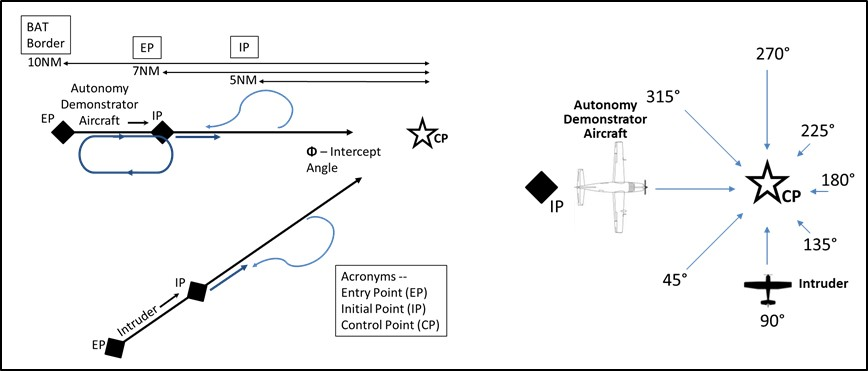
\includegraphics[width=\textwidth]{figures/flight-test.jpg}
	\caption{Flight test plan for evaluation of LEC collision avoidance and RTA safety guarantees}
	\label{fig:flight-test}
\end{figure*}

As described above, two avoidance flight plans were automatically generated on the testbed aircraft, one by the LEC and the other by the backup avoidance planner (which did not use a neural network).
The RTA architecture assessed the two plans and determined which would be flown by the testbed to remain well clear of the Intruder.

Flight testing consisted of the live execution of multiple two-aircraft test conditions.  Each test condition specified the following:
\begin{enumerate}
\item A relative heading angle between the testbed aircraft and the Intruder
\item The specification to use one of two LECs that were available on the testbed aircraft flight software
\end{enumerate}

Multiple relative heading angles were flown, including a head-on encounter (relative heading = 180 degrees), and other relative headings in 45 degree intervals.
The available LECs were termed the ``good LEC'' and the ``bad LEC.''  The ``good LEC'' was expected to generate safe remain-well-clear trajectories, while the ``bad LEC'' was designed to generate unsafe trajectories, simulating an LEC producing unintended (and unsafe) behaviors.  

During the numerous test conditions flown we made the following general observations:
\begin{itemize}
\item In test conditions where the good LEC was used, the generated avoidance flight plans resulted in safe and standards conformant remain-well-clear avoidance of the Intruder.  The RTA functionality successfully assessed the LEC plans as safe, which resulted in the testbed aircraft flying the LEC route.  
\item In test conditions where the bad LEC was used, the generated avoidance flight plans resulted in violation of the remain-well-clear avoidance criteria relative to the Intruder.  The RTA functionality successfully assessed the LEC plans as unsafe, which resulted in the testbed aircraft flying the route from the backup avoidance planner.  
\end{itemize}

%There was a case, though, where the bad LEC actually created a route good enough to be standards conformant, and the Collins RTA functionality did judge that route as safe, which resulted in the testbed aircraft flying the LEC route.

There were two interesting test conditions in which we observed unexpected results.  Recall from Section~\ref{sec:rta} that when both plans are assessed as safe but predicted CPA for either occurs at the limit of the prediction horizon, we prefer the plan whose CPA is actually within the prediction horizon.  This situation occurred spontaneously in one of our test conditions, resulting in the RTA functionality choosing (correctly) the backup plan over the LEC.  

In another test condition we were surprised to observe the RTA functionality choosing to fly the plan generated by the bad LEC.  Upon further analysis, we found that both plans were assessed as safe (though the bad LEC plan was just barely safe) and in this case the plan selector logic correctly chose the LEC plan.  However, during execution of the test scenario the RWC separation criteria was violated.  We discovered that several factors combined to place the intruder aircaft ahead of its predicted position, resulting in separation slightly below the RWC requirement.  This condition was possible in our experiment because of an initial design decision to have each of the planners produce only a single avoidance flight plan at the start of a collision encounter, with no updates for any changes that might occur during test execution.  


%For the conclusion:
%- changes/improvements for future demos (more dynamic)
% Flight Test Results
% Flight testing, results obtained for various test scenarios, and lessons learned from the demonstration [DARREN/JIM]

\section{Conclusion}

%[DARREN - 1 pg, incl refs]
%
%More dynamic RTA architecture, execute/update more frequently
%
%Multiple intruders


Our team has flight tested machine learning technology for aircraft collision avoidance with a
run-time assurance architecture designed to guarantee safety in the presence of potential
unintended behaviors.  These capabilities were integrated on Boeing's
autonomy testbed aircraft to show that they can provide correct operation and
safety guarantees needed by real aircraft.  Flight testing demonstrated the ability of the RTA
system to ensure that ``remain well clear'' separation criteria were maintained during a variety of 
collision encounter geometries.  Formal methods and an assurance argument were used to 
provide evidence of the correctness of the RTA design. 

Future work will extend the LEC planner and the RTA architecture to handle multiple intruder 
aircraft and other obstacles such as weather.  We will also update the RTA architecture to 
actively update RWC assessment during a collision encounter and dynamically request
new avoidance plans if safety has been compromised due to change in intruder aircraft behavior 
or the arrival of additional intruders.  

% next steps
% other applications?

\subsubsection*{Acknowledgment}
This work was funded by DARPA contract  FA8750-18-C-0099. The views, opinions and/or
findings expressed are those of the author and should not be interpreted as representing
the official views or policies of the Department of Defense or the U.S. Government.

\bibliographystyle{abbrv}
\bibliography{biblio}

\end{document}
